\documentclass[final]{article}

\usepackage[paper=a4paper]{geometry}
\usepackage[T1]{fontenc}
\usepackage{fourier}
\usepackage[english]{babel}
%\usepackage[utf8]{luainputenc}
%\usepackage[utf8]{inputenc}
\usepackage[fleqn]{amsmath}
\usepackage{amsthm, amssymb}
\usepackage{graphicx}

\title{%
    Saddlepoint approximations to the probability of ruin in finite time for the
    compound Poisson risk process perturbed by diffusion (Complement)%
}

\date{2014}

\author{Riccaro Gatto \and Benjamin Baumgartner}

%\usepackage[semicolon, sort&compress]{natbib}
%\bibliographystyle{agsm}

\newcommand*{\1}{\mathbb{1}}
\newcommand*{\E}{\mathbb{E}}
\newcommand*{\R}{\mathbb{R}}
\makeatletter
    \newcommand*{\diffstar}{\mathrm{d}}
    \newcommand*{\diffnostar}{\unskip{\;\mathrm{d}}}
    \newcommand*{\diff}{\@ifstar{\diffstar}{\diffnostar}}
\makeatother
\newcommand*{\e}{\mathrm{e}}
\newcommand*{\oh}{\mathrm{o}}
\newcommand*{\shift}{\ensuremath{\mathrel{\phantom{=}}\strut}}

\makeatletter
\renewenvironment{proof}[1][\proofname]{\par\pushQED{\qed}\normalfont\topsep6\p@\@plus6\p@\relax\trivlist\item[\hskip\labelsep\bfseries#1\@addpunct{.}]\ignorespaces}{\popQED\endtrivlist\@endpefalse}
\makeatother

\begin{document}
\maketitle

\section*{Introduction}

This document serves as a complement to
\begin{quote}
    [GB]\quad Gatto R.\ and Baumgartner, B. (2014).
    ``Saddlepoint approximations to the probability of ruin in finite time for the
    compound Poisson risk process perturbed by diffusion''.
    \emph{Methodology and Computing in Applied Probability}, to appear.
\end{quote}

The joint or double Laplace transform of the time of ruin $T$ and the initial capital
$Y_{0}$ is given in GB (Theorem~2.1).  A proof using the Laplace transform of the
Gerber--Shiu function is given in GB (Appendix) and a complete proof, which does not
require the Gerber--Shiu function, is the following.

\section*{Alternative proof of Theorem~2.1}
\begin{proof}[Proof of Theorem~2.1]
    Within any small time interval of length $h > 0$, either zero, one or more than one
    jumps (or claims) occur with the corresponding probabilities $1 - \lambda h + \oh(h)$,
    $\lambda h + \oh(h)$ and $\oh(h)$, as $h \downarrow 0$.  Thus, from the independence
    and the stationarity of the increments of $\{Y_{t}\}_{t \ge 0}$, we obtain
    \begin{align}
        f_{\alpha}(x)
            &= (1 - \lambda h)\,\E\E\bigl[\e^{\alpha(T + h)} \1(T < \infty) \bigm| Y_{0} = x + ch + \sigma W_{h}\bigr] \nonumber \\
                &\shift + \lambda h\,\E\E\bigl[\e^{\alpha(T + h)} \1(T < \infty) \bigm| Y_{0} = x + ch + \sigma W_{h} - X_{1}\bigr]
                        + \oh(h) \nonumber \\
            &= (1 - \lambda h)\,\e^{\alpha h}\,\E\bigl[f_{\alpha}\bigl(x + ch + \sigma W_{h}\bigr)\bigr]
                + \lambda h\,\e^{\alpha h}\,\E\bigl[f_{\alpha}\bigl(x + ch + \sigma W_{h} - X_{1}\bigr)\bigr]
                + \oh(h),
    \label{eqn:doubletransf-expsplit-as-f}
    \end{align}
    as $h \downarrow 0$ and for any $\alpha \in \R$ such that $f_\alpha(x) < \infty$.  The
    first expectation in \eqref{eqn:doubletransf-expsplit-as-f} can be written as
    \begin{align}
        \E\bigl[f_{\alpha}\bigl(x + ch + \sigma W_{h}\bigr)\bigr]
            &= f_{\alpha}(x) + \E\left[\sum_{k=1}^{2}
        \frac{f_{\alpha}^{(k)}(x)}{k!}\bigl(ch + \sigma W_{h}\bigr)^{k} + \oh \left( \{ c h + \sigma W_h \}^2
                                        \right) \right]  \nonumber\\
            &= f_{\alpha}(x) + \sum_{k=1}^{2} \left(\frac{f_{\alpha}^{(k)}(x)}{k!} \sum_{i=0}^{k} \binom{k}{i} (ch)^{k-i}\;\sigma^{i}\,\E\bigl[W_{h}^{i}\bigr]\right) + \E\left[ \oh \left( W_h^2 \right) \right] \nonumber\\
            &= f_{\alpha}(x) + ch f'_{\alpha}(x) + \tfrac{1}{2}\sigma^{2}h f''_{\alpha}(x) + \oh(h).
    \label{eqn:doubletransf-exp-taylor-one}
    \end{align}
    Similarly, the second expectation in \eqref{eqn:doubletransf-expsplit-as-f} can be
    written as
    \begin{align}
        \E\bigl[f_{\alpha}\bigl(x + ch + \sigma W_{h} - X_{1}\bigr)\bigr]
            &= \E\bigl[f_\alpha(x - X_{1})\bigr]
                + \E\left[\sum_{k=1}^{2}\frac{f_{\alpha}^{(k)}(x - X_{1})}{k!} \bigl(ch + \sigma W_{h}\bigr)^{k}
                    + \oh \left( \{ c h + \sigma W_h \}^2 \right) \right] \nonumber\\
            &= \E\bigl[f_\alpha(x - X_{1})\bigr]
                + \sum_{k=1}^{2} \left(\frac{\E\bigl[f_{\alpha}^{(k)}(x - X_{1})\bigr]}{k!} \sum_{i=0}^{k} \binom{k}{i} (ch)^{k-i}\;\sigma^{i}\,\E\bigl[W_{h}^{i}\bigr]\right)
                + \E\left[ \oh \left( W_h^2 \right) \right] \nonumber\\
            &= \E\bigl[f_{\alpha}(x - X_{1})\bigr]
                + ch\,\E\bigl[f_{\alpha}'(x - X_{1})\bigr]
                + \tfrac{1}{2}\sigma^{2}h\,\E\bigl[f_{\alpha}''(x - X_{1})\bigr] + \oh(h).
    \label{eqn:doubletransf-exp-taylor-two}
    \end{align}
    As indicated by a Referee, the existence of $f_{\alpha}''$, required in the Taylor
    expansions in \eqref{eqn:doubletransf-exp-taylor-one} and
    \eqref{eqn:doubletransf-exp-taylor-two}, is established by Feng (2011, Lemma C.1),
    because the function $f_{\alpha}$ is a special case of the more general functional of
    $T$ given in GB (Equation 15).  Replacing the expectations in
    \eqref{eqn:doubletransf-expsplit-as-f} with their respective
    expansions~\eqref{eqn:doubletransf-exp-taylor-one} and
    \eqref{eqn:doubletransf-exp-taylor-two}, dividing both sides by
        $\e^{\alpha h} h (1 - \lambda h)$
    and rearranging terms results in
    \begin{align*}
        0   &= \frac{1}{h}\Biggr(1- \frac{\e^{-\alpha h}}{1 - \lambda h}\Biggr) f_{\alpha}(x)
                + cf_{\alpha}'(x) + \tfrac{1}{2}\sigma^{2} f_{\alpha}''(x)  \\
            &\shift + \frac{1}{1 - \lambda h}\biggl(\E\bigl[f_{\alpha}(x - X_{1})\bigr]
                + ch\,\E\bigl[f_{\alpha}'(x - X_{1})\bigr] + \tfrac{1}{2}\sigma^{2}h\,\E\bigl[f_{\alpha}''(x - X_{1})\bigr]\biggr)
                + \oh(1).
    \end{align*}
    Let
        $g(h) = \e^{-\alpha h}(1 - \lambda h)^{-1}$,
    then by the rule of de l'Hospital the coefficient of $f_{\alpha}(x)$ converges to
        $\lim_{h \downarrow 0} \bigl(g(0) - g(h)\bigr) / h = -g'(0) = \alpha - \lambda$.
    Thus, by letting $h \downarrow 0$, we obtain the integro-differential equation
    \begin{align}
        0 &= \tfrac{1}{2}\sigma^{2} f''_{\alpha}(x) + cf'_{\alpha}(x)
            + (\alpha-\lambda)f_{\alpha}(x) + \lambda\,\E\bigl[f_{\alpha}(x - X_{1})\bigr]
    \nonumber \\ \intertext{or, equivalently,}
        0 &= \tfrac{1}{2}\sigma^{2} f''_{\alpha}(x)
            + cf'_{\alpha}(x)
            + (\alpha-\lambda)f_{\alpha}(x)
            + \lambda \int_{0}^{x} f_{\alpha}(x-\xi)\diff F_{X}(\xi)
            + \lambda[1 - F_{X}(x)].
    \label{eqn:intdiffeq}
    \end{align}

    In the next step, both sides of \eqref{eqn:intdiffeq} are multiplied by $\e^{\beta x}$
    and integrated from $0$ to $\infty$.  This corresponds to taking Laplace transforms
    with reversed sign of the argument $\beta$, thus
        $\smash{\widehat{f_{\alpha}'}}(\beta) = -\beta \hat{f}_{\alpha}(\beta) - f_{\alpha}(0)$
    and
        $\smash{\widehat{f_{\alpha}''}}(\beta) = \beta^{2} \hat{f}_{\alpha}(\beta) + \beta f_{\alpha}(0) - f_{\alpha}'(0)$,
    for any $\beta \in \R$ such that $\hat{f}_\alpha(\beta) < \infty$, where
        $\hat{g}(u) = \int_0^\infty \e^{u x} g(x) \diff x$,
    for a generic function $g$.  As a consequence,
    \begin{align*}
        0   &= \tfrac{1}{2}\sigma^{2} \bigl[\beta^{2}\hat{f}_{\alpha}(\beta) + \beta f_{\alpha}(0) - f'_{\alpha}(0)\bigr]
                + c\bigl[-\beta \hat{f}_{\alpha}(\beta) - f_{\alpha}(0)\bigr] \\
            &\shift + (\alpha - \lambda) \hat{f}_{\alpha}(\beta)
                + \lambda \hat{f}_{\alpha}(\beta) M_{X}(\beta) - \tfrac{\lambda}{\beta} \bigl[1 - M_{X}(\beta)\bigr],
    \end{align*}
    which, when solved for $\hat{f}_{\alpha}(\beta)$, which is the left-hand
    side of \eqref{eqn:double-laplace-transform}, leads to
    \begin{align*}
        \hat{f}_{\alpha}(\beta)
            &= \frac{%
                \bigl(c - \frac{1}{2}\sigma^{2}\beta\bigr) f_{\alpha}(0)
                + \tfrac{1}{2}\sigma^{2} f'_{\alpha}(0)
                - \tfrac{\lambda}{\beta} \bigl(M_{X}(\beta) - 1\bigr)
            }{%
                \tfrac{1}{2}\sigma^{2}\beta - c\beta + \alpha + \lambda \bigl(M_{X}(\beta) - 1\bigr)
            }\\
            &= \frac{%
                \bigl(c - \tfrac{1}{2}\sigma^{2}\beta\bigr) f_{\alpha}(0)
                + \tfrac{1}{2}\sigma^{2} f'_{\alpha}(0)
                - \frac{\kappa(\beta)}{\beta} + \tfrac{1}{2}\sigma^{2}\beta - c
            }{%
                \kappa(\beta) + \alpha
            }.
    \end{align*}

    Note that $\hat{f}_{\alpha}(\beta)$ exists for all $\beta < 0$, if $\alpha < 0$.  In
    particular, it exists for $\beta = v(\alpha) < 0$ with $\alpha < 0$.  In this case the
    above denominator vanishes and therefore $v(\alpha)$ is a common root of both the
    denominator and numerator above, otherwise the existence of
    $\hat{f}_{\alpha}(v(\alpha))$ would be contradicted.  Because of that, setting the
    numerator equal to $0$ and substituting $v(\alpha)$ for $\beta$ yields
    \begin{equation*}
        \tfrac{1}{2}\sigma^{2} f'_{\alpha}(0) =
            - \bigl(c - \tfrac{1}{2}\sigma^{2} v(\alpha)\bigr)\;f_{\alpha}(0)
            - \frac{\alpha}{v(\alpha)} - \tfrac{1}{2}\sigma^{2} v(\alpha) + c,
    \end{equation*}
    and hence
    \begin{equation*}
        \hat{f}_{\alpha}(\beta) = \frac{%
            \frac{1}{2}\sigma^{2} \bigl(\beta - v(\alpha)\bigr) \bigl(1 - f_{\alpha}(0)\bigr)
            - \frac{\kappa(\beta)}{\beta} - \frac{\alpha}{v(\alpha)}
        }{%
            \kappa(\beta) + \alpha
        }.
    \end{equation*}
    Without initial reserve, i.\,e.\ for $x = 0$, ruin occurs almost surely and $T = 0$
    a.\,s.\ because the regularity of the Wiener process implies that the risk process
    crosses the null level infinitely often over any arbitrarily small time interval
    containing the origin.  Hence $f_{\alpha}(0) = 1$ and, as a consequence, GB (Equation
    12), i.\,e.
    \begin{equation}
        \hat{f}_{\alpha}(\beta) =
            -\frac{
                \frac{\alpha}{v(\alpha)} + \frac{\kappa(\beta)}{\beta}
            }{
                \alpha + \kappa(\beta)
            }
    \label{eqn:double-laplace-transform}
    \end{equation}
    holds for all $\alpha, \beta < 0$.

    From the fact that
        $D = \{(\alpha, \beta) \in \R^{2}\colon \alpha \le \mathring{\alpha},\ \beta < \tilde{v}(\alpha)\}$
    is a connected subset of $\R^{2}$ and the right-hand side of
    \eqref{eqn:double-laplace-transform} is an analytical function for all $\alpha, \beta
    \in D$, follows that the double Laplace transform
    formula~\eqref{eqn:double-laplace-transform} holds over the entire set $D$.
\end{proof}

A helpful picture of the domain $D$ is given by Figure \ref{f1}.
\begin{figure}[htbp]
    \centering
    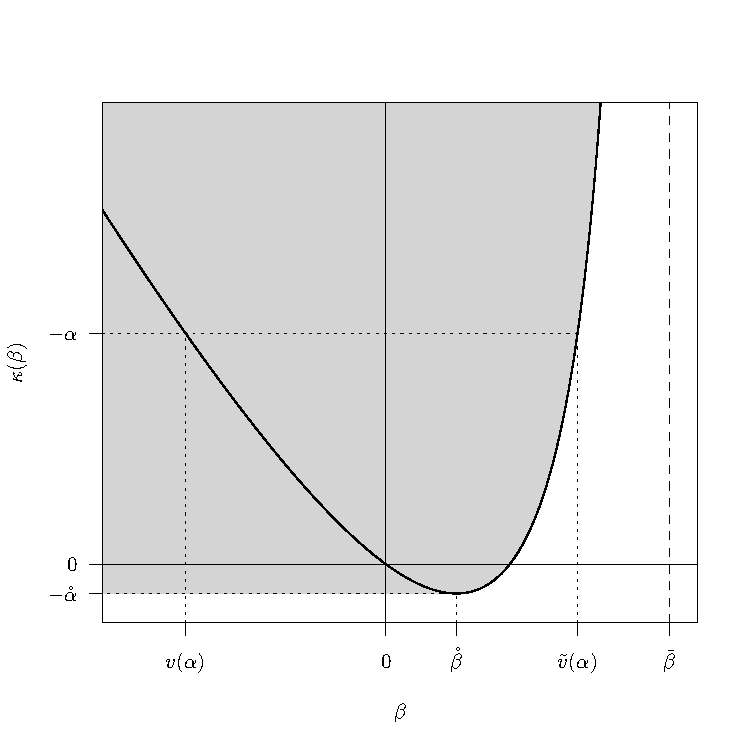
\includegraphics[width=0.7\linewidth]{domain.pdf}
    \caption{A representation of the domain $D$ of the double Laplace transform
        $\hat{f}_{\alpha}(\beta)$}
    \label{f1}
\end{figure}


\end{document}
